\section{Moderne Enterprise-Architektur}

%%%%%%%%%%%%%%%%%%%%%%%%%% Microkernel Architecture %%%%%%%%%%%%%%%%%%%%%%%%%%%

\begin{frame}{Microkernel Architecture}
    \begin{itemize}
        \item Aufteilung der Anwendung in zwei Komponenten~\cite{architecturePatterns}
        \item Kern:
        \begin{itemize}
            \item Minimale Funktionalität
            \item Bietet Schnittstelle für Erweiterungen/Plugins
            \item Enthält Plugin-Registry
        \end{itemize}
        \item Module:
        \begin{itemize}
            \item Erweitern Kern um Funktionalitäten
            \item Kommunikation über definierte Schnittstellen
            \item Lose gekoppelt, unabhängig und isoliert voneinander
            \item Verbindung über verschiedene Wege möglich (REST, Messaging, Objekt Instanziierung, \ldots)
            \end{itemize}
    \end{itemize}
\end{frame}

\begin{frame}{Microkernel Architecture: Struktur}
    \begin{figure}[!h]
        \centering
        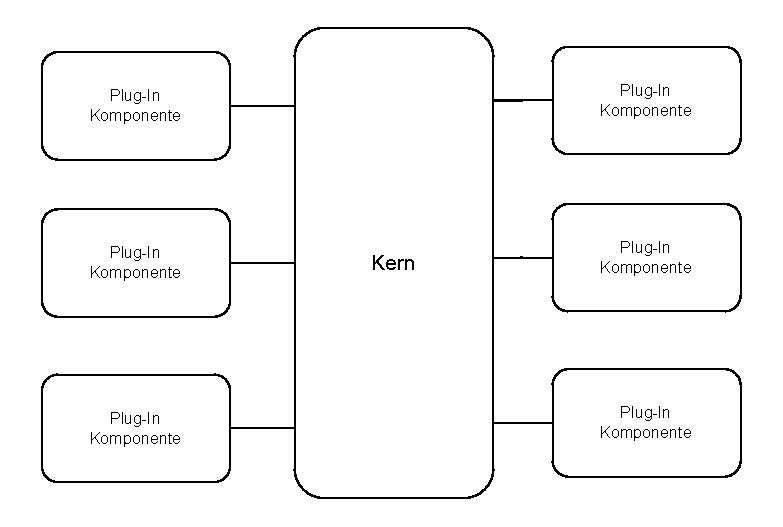
\includegraphics[scale=0.55]{imglib/microkernel/microkernel}
        \caption{Aufbau einer Microkernel Architecture}
        \label{fig:microkernel}
    \end{figure}
\end{frame}

\begin{frame}{Microkernel Architecture: Beispiel E-Commerce I}
    \begin{itemize}
        \item Kern: Großteil der Funktionalität
        \item Module: Auslagerung von Business-Logik zum Bezahlen und Versenden
        \item Einfache Erweiterbarkeit durch neue Dienstleister
        \item Komplexer Kern, hohe Kopplung der übrigen Funktionalitäten
        \item Als einziges Architekturmuster eher nicht geeignet, jedoch in Kombination mit anderen sinnvoll
    \end{itemize}
\end{frame}

\begin{frame}{Microkernel Architecture: Beispiel E-Commerce II}
    \begin{figure}[!h]
        \centering
        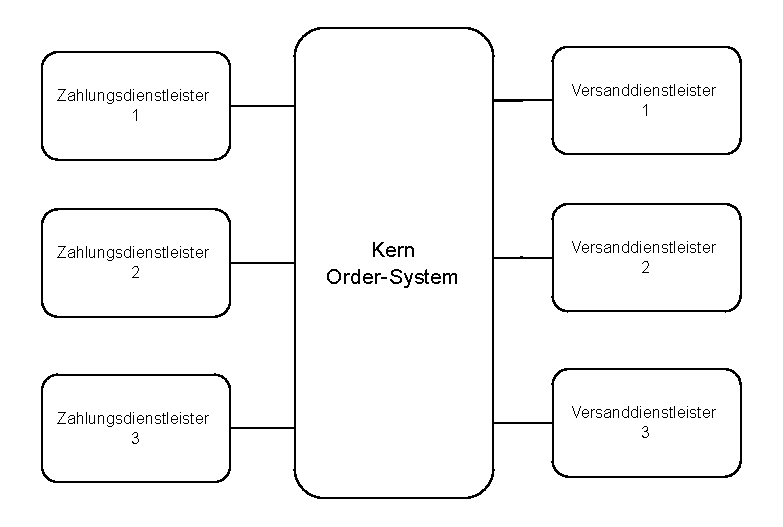
\includegraphics[scale=0.55]{imglib/microkernel/ecommerce-microkernel}
        \caption{E-Commerce-Beispiel mit Microkernel Architecture}
        \label{fig:microkernel-ecommerce}
    \end{figure}
\end{frame}

\begin{frame}{Microkernel Architecture: Agilität}
    \begin{itemize}
        \item Lose Kopplung der Module $\Rightarrow$ schnelle Reaktionsfähigkeit auf Änderungen
        \item Module können einfach ausgetauscht werden $\Rightarrow$ geringe Downtime
        \item Einfach testbar, da Module unabhängig und isoliert voneinander
        \item Kurze Iterationen und Auslieferungszeiten bei Erweiterung der Anwendung
        \item Aber: Hoher initialer Aufwand durch teuren Kern, eher hohe Time-to-Market
        \item Aber: Hoher Aufwand, wenn Kern später Anpassungen benötigt
        \item Fazit: In ausgewählten Anwendungsfällen sinnvoll, aber nicht universell in agilen Umgebungen einsetzbar
    \end{itemize}
\end{frame}

%%%%%%%%%%%%%%%%%%%%%%%%%% Event-Driven Architecture %%%%%%%%%%%%%%%%%%%%%%%%%%

\begin{frame}{Event-Driven Architecture}
    \begin{itemize}
        \item Bisher: Expliziter Aufruf von Funktionalitäten
        \item Jetzt: Impliziter Aufruf durch Reaktion auf Ereignisse \cite{garlanShawImplizit}
        \item System reagiert asynchron auf Zustandsänderung (Ereignis in System)
        \item Alte Idee: David Garlan und Mary Shaw, 1994, \textit{An Introduction to Software Architecture}
    \end{itemize}
\end{frame}

\begin{frame}{Event-Driven Architecture: Komponenten}
    \begin{itemize}
        \item Event: Kapselt Information einer Zustandsänderung eines Systems \cite{eda}
        \item Produzent: Erzeugt Event
        \item Publisher: Publiziert erzeugtes Event
        \item Konsument: Reagiert auf Event
        \item Mediator: Vermittler zwischen Produzenten und Konsumenten
        \item Event-Broker: Infrastruktur für Gesamtheit der Vermittler
    \end{itemize}
\end{frame}

\begin{frame}{Event-Driven Architecture: Struktur}
    \begin{figure}[!h]
        \centering
        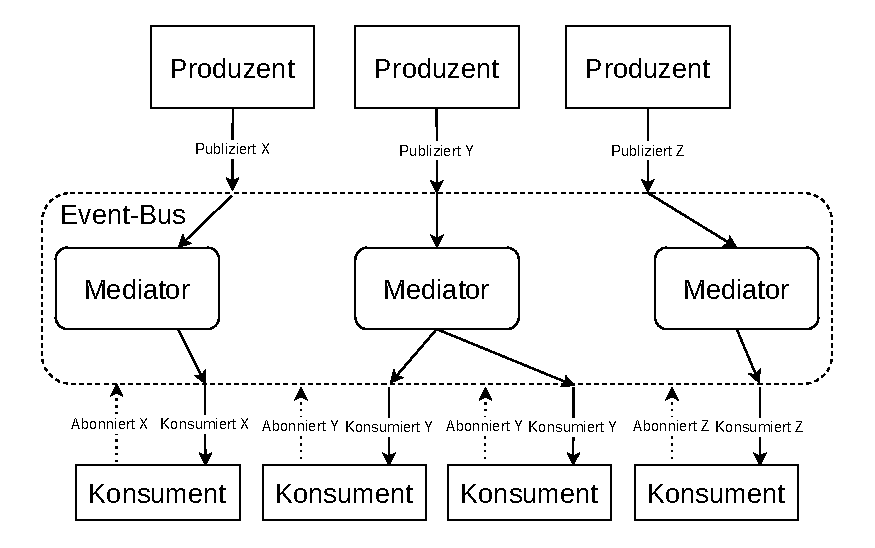
\includegraphics[scale=0.55]{imglib/eda/eda.drawio}
        \caption{Vertrag zwischen Produzenten und Konsumenten am Event-Bus}
        \label{fig:eda}
    \end{figure}
\end{frame}

\begin{frame}{Event-Driven Architecture: Beispiel E-Commerce I}
    \begin{itemize}
        \item \texttt{OrderCreated}: Genau dann, wenn Bestellung aufgegeben wird
        \item \texttt{PaymentProcessed}: Genau dann, wenn Bezahlvorgang abgeschlossen wird
        \item \texttt{ShipmentInitiated}: Genau dann, wenn Bestellung versandt wird
        \item Event-Kette: $ \texttt{OrderCreated} \rightarrow \texttt{PaymentProcessed} \rightarrow \texttt{ShipmentInitiated}$
        \item Implementierung in Diensten: OrderService, PaymentService, ShipmentService
    \end{itemize}
\end{frame}

\begin{frame}{Event-Driven Architecture: Beispiel E-Commerce II}
    \begin{figure}[!h]
        \centering
        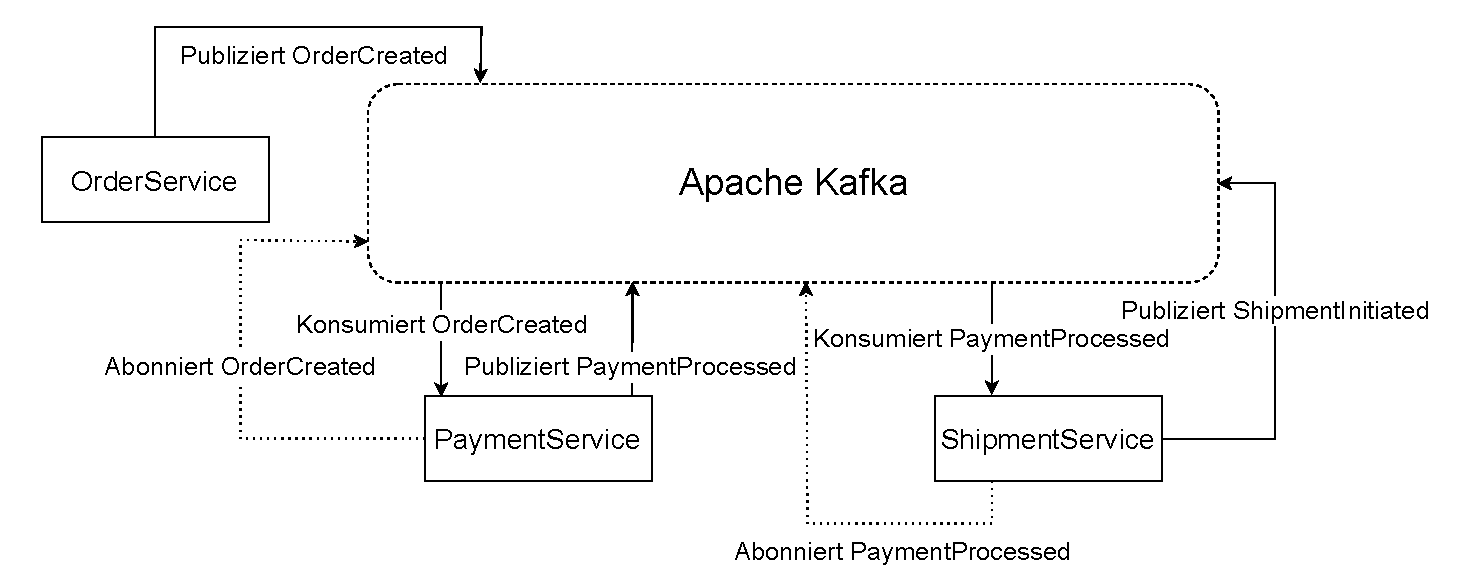
\includegraphics[scale=0.5]{imglib/eda/eda-ecommerce.drawio}
        \caption{E-Commerce-Beispiel mit Event-Driven Architecture}
        \label{fig:edaecommerce}
    \end{figure}
\end{frame}

\begin{frame}{Event-Driven Architecture: Agilität}
    \begin{itemize}
        \item Event ist Vertrag zwischen Produzent und Konsument am Event-Broker\\
        $\Rightarrow$ Hohe Kohäsion $\Rightarrow$ Lose Kopplung
        \item Feature: Menge von Events, deren Produzenten und Konsumenten\\
        $\Rightarrow$ Klare Abgrenzung $\Rightarrow$ einfach definierbare Iterationen
        \item Events sind sehr realitätsnah - domain-driven
        \item Sehr hohe Flexibilität \& maximale Skalierung durch lose Kopplung
        \item Schnelle Auslieferung, kurze Intervalle
        \item Exzellente Kombination mit Microservices \& Cloud-Integration
        \item Aber: Erhöhte Komplexität $\Rightarrow$ Hohe Anforderungen an Entwickler
    \end{itemize}
\end{frame}

%%%%%%%%%%%%%%%%%%%%%%%%%% Cloud-Native Architecture %%%%%%%%%%%%%%%%%%%%%%%%%%

\begin{frame}{Cloud-Native Architecture}
    \begin{itemize}
        \item Bisher: Vorab-Allokation von Ressourcen
        \item Jetzt: Allokation genau dann, wenn notwendig
        \item Cloud-Native: Explizit für die Cloud entwickelte Applikationen \cite{cloudNative}
        \item Annahme: Infrastruktur ist in ständigem Wandel
        \item Folgerung: Infrastruktur auslagern - an Cloud-Vendor
        \begin{itemize}
            \item Globale Nutzung durch Geo-Redundanz: Starke Verteilung und hohe Verfügbarkeit
            \item Auto-Scaling: Dynamische Skalierung basierend auf Nachfrage
            \item Pay-as-you-go, Scale-to-zero: Nur verwendete Ressource wird bezahlt
            \item Zero Downtime
        \end{itemize}
    \end{itemize}
\end{frame}

\begin{frame}{Cloud-Native Architecture: Technologie}
    \begin{itemize}
        \item Containerisierung: Jede Komponente eines Systems ist Container
        \item Dynamische Orchestrierung: Aktives Container-Management zur Ressourcenoptimierung
        \item Microservice-Architektur ist Fundament - ergänzt durch Cloud-Dienste
        \item Fully Managed Cloud-Services: Business-Logik statt Infrastruktur
    \end{itemize}
\end{frame}

\begin{frame}{Cloud-Native Architecture: Beispiel E-Commerce}
    \begin{figure}[!h]
        \centering
        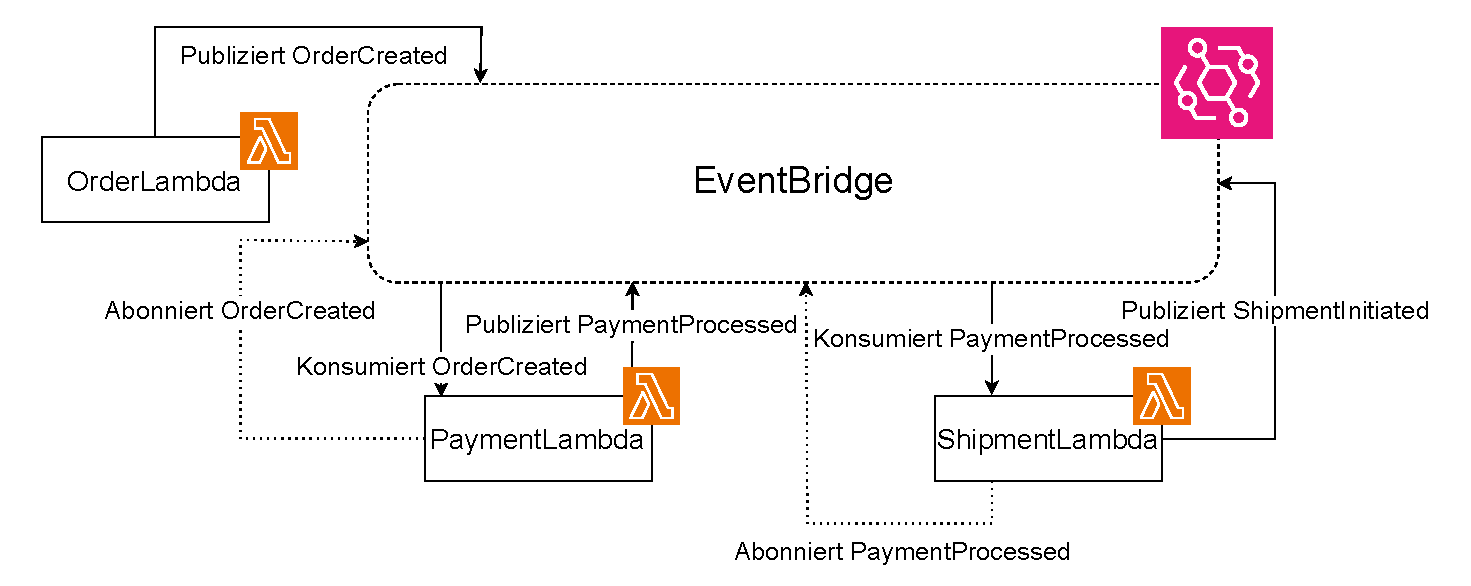
\includegraphics[scale=0.5]{imglib/cloud-native/cloud-native-ecommerce.drawio}
        \caption{E-Commerce-Beispiel mit Cloud-Native Architecture in AWS}
        \label{fig:cloudnativeecommerce}
    \end{figure}
\end{frame}

\begin{frame}{Cloud-Native Architecture: Agilität}
    \begin{itemize}
        \item Alle agilen Vorteile von Microservice- und Event-Driven Architecture
        \item Fokus auf Business-Logik \& einfaches Deployment $\Rightarrow$ Kurze Iterationen
        \item Maximale Flexibilität für Nachfrage durch Auto-Scaling
        \item Finanzielle Agilität: Pay-as-you-go
        \item Aber: Kostenrisiken durch Auto-Scaling und Pay-as-you-go
        \item Achtung: Vendor-Lock-In durch proprietäre Fully Managed Cloud-Services
    \end{itemize}
\end{frame}